\sinote{Intro mangler. Brug \cref{fig:pact-overview}}

\begin{figure}
  \centering
  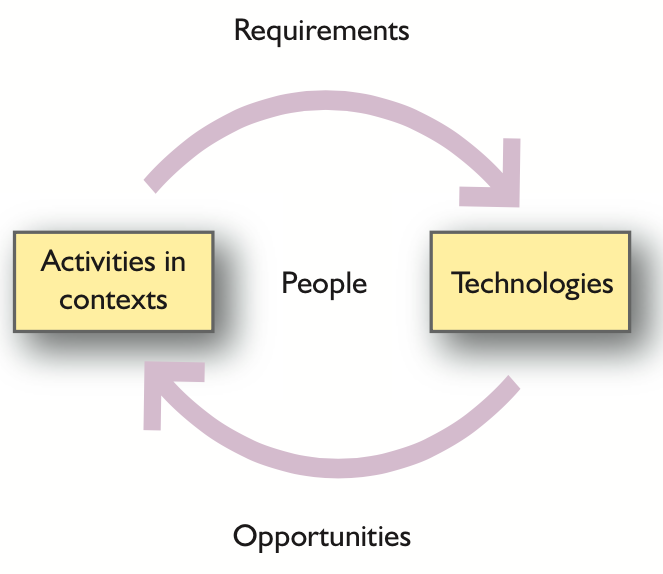
\includegraphics[width=0.5\linewidth]{pact-overview.png}
  \caption{The relationships between activities, contexts, people and technologies in PACT. From \cite{benyon2013designing}}
  \label{fig:pact-overview}
\end{figure}

\subsection{People}
\label{sub:pact_people}

The system is used by people who go to bar-like environments, and are possibly intoxicated. At bar-like environments, music is central to the atmosphere, and a lot of people are interested in having their music tastes accommodated. Different people exhibit different behaviour in these social contexts, some may clique together when using a social system and some may be afraid of stigmas when using it. To use the system, a smartphone is required, and some people may be unable or afraid to use their smartphone.

\subsection{Activities}
\label{sub:pact_activities}

Usage of the system requires the user to interact with their smartphone or similar device. Firstly the user must install the application on their device and sign in using their Facebook or Google account. When the user has signed in to the application, they will either have to go to the voting screen or request screen. When in the voting screen, the user can press an upvote button or downvote button for each song in the playlist. In the request screen, users can browse the available library, find a song they like and add it to the playlist.

\subsection{Context}
\label{sub:pact_context}

This system can be used at places where many people wants to listen to music, but does not have an efficient method of determining which songs to listen to.

A dark environment with a lot of noise is common in bars/pubs. As people are often dancing in this environment, active use of smartphones is not recommended. Also, usage of smartphones in these kind of environments often cause anti-social behavior.

\subsection{Technologies}
\label{sub:pact_technologies}

The system runs on a host computer with an audio system connected and a business license for Spotify. This host computer is located at the installation site. 

For users to operate this system a smartphone with internet connection and adequate battery life is required. Login to the system requires a Facebook/Google account.

When designing the system, different smartphones and their characteristics have to be considered.
